%!TEX ROOT=ctutest.tex

\chapter{Reinforcement Learning}
\label{chapter:rl}

Reinforcement learning (RL) is an area of machine learning inspired by behaviorist psychology, concerned with how software agents ought to take actions in an environment so as to maximize some notion of cumulative reward. The problem, due to its generality, is studied in many other disciplines, such as game theory, control theory, operations research, information theory, simulation-based optimization, multi-agent systems, swarm intelligence, statistics, and genetic algorithms. 

Reinforcement learning differs from standard supervised learning in that correct input/output pairs are never presented, nor sub-optimal actions explicitly corrected. Further, there is a focus on on-line performance, which involves finding a balance between exploration (of uncharted territory) and exploitation (of current knowledge) \cite{cite:wiki-rl}.

In machine learning, the environment is typically formulated as a Markov decision process (MDP). The main difference between classical techniques and reinforcement learning algorithms is that the latter do not need knowledge about the MDP and they target large MDPs where exact methods become infeasible.

\section{Introduction}
The basic RL model consists of:
\begin{itemize}
\item a state in a set of environment states $\textit{s} \in \textbf{\textit{S}}$
\item an action in a set of actions $\textit{a} \in \textbf{\textit{A}}$
\item rules of transitioning between states $s_t\to s_{t+1}$

\item rules that determine the scalar immediate reward $r \in \mathbb{R}$ of a transition
\end{itemize}
The rules are often stochastic, especially the rules of state transitioning. Depending on the type of the problem, we divide the MDPs to fully observable (agent has full access to all information about the state) and partially observable (some information about the state is not available).

A RL agent interacts with the environment at discrete time-steps, observing the state $s_t$ by receiving an observation $o_t$\footnote{To simplify notation, we further consider $o_t\equiv s_t$} and typically a reward $r_t$. The agent then chooses an action $a_t$ which is 'sent' to the environment. The environment moves to another state $s_t\to s_{t+1}$.

The goal of a RL agent is to collect as much reward as possible.

\begin{figure}
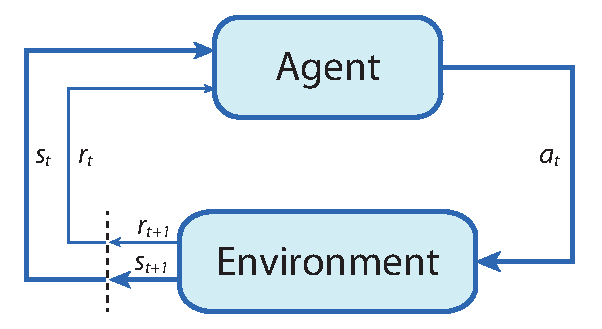
\includegraphics[width=\textwidth*\real{0.8}]{images/rl/rl_loop_blue.pdf}
\caption{Interaction of a RL agent with the environment}
\end{figure}

\subsection{Policy}
A policy $\pi$ is used to pick actions in the MDP. In general, the policy is stochastic and denoted by $\pi_\theta: S \to P(A)$ where $\theta \in \mathbb{R}^n$ is the parameter vector and $\pi_\theta(a|s)=\mathbb{P}[a|s;\theta]$ selects an action according to some probability measure $P(A)$.

\subsection{Reward}
The reward in time-step $t$ is a function $r_t(s_t,a_t)$ that returns the immediate reward of the transition $s_t\to s_{t+1}$.
The return $R_t^\gamma$ is the total discounted reward from time step $t$ onward.

\begin{equation}
R_t^\gamma=\sum_{k=t}^\infty \gamma^{k-t}r(s_k,a_k)
\end{equation}

$\gamma \in \left\langle 0,1\right\rangle$ is a coefficient capturing how much do we care about events in the far future\footnote{$\gamma=0$ means we only care about the immediate reward, $\gamma=1$ means the value should depend on the future fully. This value is often close to $1$ and is task-dependent.}.

The goal of a RL agent is to find a policy that maximizes the expected cumulative reward from the start state, denoted by the objective function

\begin{equation}
J(\pi)=\mathbb{E}[R_0^\gamma|s_0;\pi]
\end{equation}
We denote the probability density at state $s_{t+k}$ after transitioning for $k$ time steps from state $s_t$ as $p(s_t\to s_{t+k},k,\pi)$. We also denote the discounted state distribution as $\rho^\pi(s_{t+k})=\int_S\sum_{t=1}^\infty \gamma^{k-1}p(s_{t})$


\subsection{Finite differences}
I would like to mention one extremely simple RL approach. Let's assume we have an agent $\mu_theta(s_t)=a_t$ (doesn't have to be deterministic).

By using finite gradient differences, we can approximate gradients of the objective function as:
\begin{equation}
\dfrac{\partial J}{\partial \theta} \approx \dfrac{J(\theta + \epsilon)-J(\theta)}{\epsilon}
\end{equation}

This means we have to run a sample episode for each parameter we want to update. This makes this method highly inefficient, however when using agents with very few parameters, even this method has some practical uses (demonstrated for example on the AIBO robots, where it was used to speed up the walking process).

I have tried this method on the network learned in chapter \ref{chapter:sl}. The robot was actually learning to move faster, until a certain point where it became unstable.

\subsection{Action-Value function}
A \textit{value function} is a function defined as the expected total discounted reward from state $s_t$ when picking actions according to the policy $\pi$.

\begin{equation}
V^\pi(s_t)=\mathbb{E}[R_t^\gamma|s_t;\pi]
\end{equation}

An \textit{action-value function} inputs a state and an action and outputs the expected return from state $s_t$ after taking action $a_t$ and afterwards picking actions according to the policy $\pi$.

\begin{equation}
Q^\pi(s_t,a_t)=\mathbb{E}[R_t^\gamma|s_t, a_t;\pi]
\end{equation}

This difference may seem subtle, but is significant. It is common practice to pick actions that maximize the expected return - this would be impossible with the simpler value function.

\section{Action-Value function approximation}

The common approaches used for model-free value function approximation are:

\begin{itemize}
\item \textbf{Monte Carlo Methods:} Applicable only for episodic problems, the values of $V(s_t)$ are updated in the direction of the total reward seen when starting from state $s_t$. Given enough time, this procedure can construct a precise estimate of the $V$ value.

\begin{equation}
V(s_t)\leftarrow V(s_t)+\alpha (R_t-V(s_{t+1}))
\end{equation}

$R_t$ is the actual return, $\alpha$ some learning constant.

MC methods however work effectively only for small MDPs and are overall slow.

\item \textbf{Temporal Difference Methods:} TD methods deal with the limiting character of the MC methods by using it's own estimates to correct itself.

\begin{equation}
V(s_t)\leftarrow V(s_t)+\alpha (r_{t+1}+\gamma V(s_{t+1})-V(s_t))
\end{equation}

$r_{t+1}+\gamma V(s_{t+1})$ is the estimated return.
\end{itemize}

\subsection{Q-learning}
Q-learning is an extension of TD learning that can be used for learning the action-value function. It simplifies the action policy dynamic by eliminating the policy from the equation and chooses actions that maximize the predicted reward. See \ref{algo:q-learning}.

\begin{algorithm}[h]
  \caption{Q-learning algorithm}
  \begin{algorithmic}
    \STATE Initialize $Q$-values arbitrarily for all state-action pairs.
    \FOR{each step}
      \STATE Choose an action $a_t = \text{argmax}_a Q(s_t, a)$
      \STATE Execute action $a_t$, observe reward $r_t$ and observe new state $s_{t+1}$
      \STATE Update $Q(s_t,a_t) = Q(s_t,a_t)+\alpha[r_t + \text{argmax}_a Q(s_{t+1}, a) - Q(s_t,a_t)] $
    \ENDFOR
  \end{algorithmic}
  \label{algo:q-learning}
\end{algorithm}
When dealing with small MDPs, it is possible to store the action-value values in a lookup table. This becomes unfeasible with larger MDPs and requires the use of a function approximator. Neural networks are a natural choice for this task, because they can capture highly non-linear relationships between inputs and outputs of the a-v function.
\medskip

Directly implementing Q-learning with neural networks proved to be unstable in many environments. Since the network being updated is also used for calculating the target value, the Q updates are prone to divergence. 

These methods, combined with actor-critic algorithms were used successfully on state-spaces with lower dimensions, however struggled when applied to high state space domains. This changed in 2015 when \cite{cite:atari} successfully applied modified Q-learning algorithm on the Atari domain.


\section{Deep Q-learning}
The deep Q-learning algorithm (DQN) has been the first algorithm capable of solving array of diverse and challenging tasks. The tasks, without going to too much detail, were to maximize the game score on several different Atari games. The inputs to the systems were pixels a human would see when playing the games. The outputs were several different actions a human could take by using a controller (like up, down, etc..).

Convolutional neural networks followed by fully connected layers were used as the action-value function approximator.
The algorithm therefore combines reinforcement learning with deep learning.

 What made the algorithm stable compared to past attempts, were two main changes over the previously used Q-learning algorithm. The Q-learning used a replay buffer and a so-called target network. 
\begin{itemize}

\item \textbf{Replay buffer:} The algorithm uses a large replay buffer from which it uniformly samples a minibatch each step of the learning process. This shift from online to batch learning has lowered the correlation of learned samples and as such has brought the most significant performance improvement.

\item \textbf{Target network:} Another previously unutilized method is the addition of another neural network - a copy of the main one. The other network is not updated each learning step, it is instead updated less often with the original network weights. This brings the learning process closer to supervised learning for which robust solution exists.
\end{itemize}

See \ref{algo:dqn} for the complete algorithm.
\begin{algorithm}[h]
  \caption{Deep Q-learning algorithm \label{algo:dqn}}
  \label{algo:dqn}
  \begin{algorithmic}
    \STATE Randomly initialize action-value function $Q$ with weights $\theta^{Q}$.
    \STATE Initialize target network $Q'$ with weights $\theta^{Q'}
    \leftarrow \theta^{Q}$
    \STATE Initialize replay buffer $R$
    \FOR{episode = 1, M}
      \STATE Receive initial observation state $s_1$
      \FOR{t = 1, T}
        \STATE With probability $\epsilon$ select a random action $a_t$,\\
        otherwise select $a_t = \text{argmax}_a Q(s_t, a_t)$
        \STATE Execute action $a_t$, observe
        reward $r_t$ and observe new state $s_{t+1}$
        \STATE Store transition $(s_t, a_t,
                r_t, s_{t+1})$ in $R$
        \STATE Sample a random minibatch of $N$ transitions
               $(s_t, a_t, r_t, s_{t + 1})$ from $R$
        \STATE Set $ y_t = 
        \begin{cases}
            r_t + \gamma Q'(s_{t + 1}, a_{t+1}) &
                                  \text {for non terminal state} \\
                                  r_t & \text{for terminal state} \\
            \end{cases} $
        \STATE Update $Q$ by minimizing the loss:
               $L = \frac{1}{N} \sum_i (y_t -
               Q(s_t, a_t | \theta^Q))^2$
        \STATE Every C steps update the target networks: $\theta^{Q'} \leftarrow \theta^{Q}$
        \ENDFOR
    \ENDFOR
  \end{algorithmic}
\end{algorithm}

DQN was able to solve a set of complex problems in continuous state space domain, however the action domain consisted of only a few discrete actions. 

The DDPG algorithm was able to combine deep Q-learning with actor-critic algorithms to overcome this limitation.

\section{Actor-Critic Algorithms}
Picking the actions that maximize the future rewards lays hard requirements on the AVF approximator. It is easy to imagine that even minor changes to the function's parameters will change the best action dramatically (because max only cares about the absolute values).

The \textit{actor-critic} (see \ref{algo:actor-critic}) is an extension of the ideas introduced by Q-learning and eases these requirements. Instead of picking the actions that maximize the future rewards (and effectively removing the actor from the equation), an actor network is introduced for picking the actions independently from the critic $Q$ network.

It is a widely used architecture based on the policy gradient theorem used for stochastic policies

\begin{equation}
\begin{split}
\nabla_\theta J(\pi_\theta)=\int_S \rho^\pi(s) \int_A \nabla_\theta \pi_\theta(a|s)Q^\pi(s,a)\text{d}a\text{d} s=\\
\mathbb{E}_{s\sim\rho^\pi, a\sim\pi_\theta}[\nabla_\theta \log \pi_\theta(a|s)Q^\pi(s,a)]
\end{split}
\label{eq:policy-gradient-theorem}
\end{equation}

The algorithm consists of two crucial components. 

The \textit{actor} $\pi(s)$ is used for picking actions each time step and learns by gradient ascent of equation \ref{eq:policy-gradient-theorem}.

The \textit{critic} $Q^\pi(s,a)$ is used for AVF approximation.

\begin{algorithm}[h]
  \caption{Actor-Critic algorithm \label{algo:actor-critic}}
  \label{algo:actor-critic}
  \begin{algorithmic}
    \STATE Initialize critic $Q(s, a | \theta^Q)$ and actor
    $\pi(s | \theta^{\pi})$ with weights $\theta^{Q}$ and $\theta^{\pi}$.
    \STATE Observe initial state $s_t$
    \FOR{each step}
      \STATE Choose an action $a_t = \pi(s_t)$
      \STATE Execute action $a_t$, observe reward $r_t$ and observe new state $s_{t+1}$
      \STATE $y=r_t+Q(s_{t+1},\pi(s_{t+1}))$
      
      \STATE $\theta^Q \leftarrow \theta^Q-\alpha\nabla_{\theta^Q}\left(y-Q(s_t, a_t)\right)^2$
      \STATE $\theta^\pi \leftarrow \theta^\pi+\alpha\nabla_{\theta^\pi}J$
    \ENDFOR
  \end{algorithmic}
\end{algorithm}


\subsection{Deterministic Policy Gradient}
Formerly mentioned methods have been used for stochastic policies in the past. For some tasks however, specifically continuous control (like walking), it doesn't make much sense to consider stochastic action-picking.

Recently, Silver et al \cite{cite:DPG} proved that the deterministic policy gradient exists (it was previously thought it doesn't) and has the simple form of 
\begin{equation}
\begin{split}
\nabla_\theta J(\mu_\theta)= \int_S \rho^\mu(s) \nabla_\theta \mu_\theta(s) \nabla_aQ^\mu(s,a)|_{a=\mu_\theta(s)}\text{d}s=\\
\mathbb{E}_{s\sim\rho^\mu}[\nabla_\theta \mu_\theta(s) \nabla_aQ^\mu(s,a)]
\end{split}
\end{equation}


